\section{Ejercicio 3}
En este ejercicio se corre el siguiente programa.

\lstinputlisting[language={[Motorola68k]Assembler}]{code/ej3.asm}


Teniendo en cuenta el siguiente estado inicial en los registros.

$$ a = \$00a00000000000 $$
$$ y = \$000000000000 $$
$$ ccr = \$00 $$

A continuación se muestra un desglose del programa, indicando aquellos registros que cambian a medida que este se ejecuta.

\begin{table}[H]
\centering
\begin{tabular}{|c|c|c|}
\hline
\textbf{Instrucción} & \textbf{Cambios}                                                                                                                  & \textbf{Comentarios}                                                                                                                                                                                                                          \\ \hline
-                  & \begin{tabular}[c]{@{}c@{}}a = \$00a00000000000\\ x = \$xxxxxxxxxxxx\\ y = \$000000000000\\ r7 = \$xxxx\\ ccr = \$00\end{tabular} & Carga inicial de valores.                                                                                                                                                                                                                     \\ \hline
move a1,x1           & \begin{tabular}[c]{@{}c@{}}x = \$a00000xxxxxx\\ ccr = \$00\end{tabular}                                                           & \begin{tabular}[c]{@{}c@{}}Carga de a1 (\$a00000) en x1.\end{tabular}                                                                                    \\ \hline
move a,y1            & \begin{tabular}[c]{@{}c@{}}y = \$7fffff000000\\ ccr = \$40\end{tabular}                                                           & \begin{tabular}[c]{@{}c@{}}Se interpreta al registro a como punto fijo.\\ a = 1,25. \\ Se produce overflow.\\ Se redondea y1 al máximo numero positivo representable.\\ En el CCR, se activa el bit \textit{Limit} (L=1) indicando lo anterior\end{tabular} \\ \hline
move a,r7            & \begin{tabular}[c]{@{}c@{}}r7 = \$ffff\\ ccr = \$40\end{tabular}                                                                  & \begin{tabular}[c]{@{}c@{}}Al mover el acumulador a a r7, se produce overflow.\\ Como r7 es entero, se interpreta a a como entero.\\ Se redondea r7 al máximo valor representable (\$ffff)\end{tabular}                                       \\ \hline
move a1,x0           & x = \$a00000a00000                                                                                                                & \begin{tabular}[c]{@{}c@{}}En este caso se realiza una operación de copia de registro.\\ No se interpreta el número como punto fijo.\end{tabular}                                                                                             \\ \hline
\end{tabular}
\caption{Paso a paso de las instrucciones ejecutadas.}
\label{tab:ej3_instructions}
\end{table}

En la tabla~\ref{tab:ej3_results} se muestra el estado final de los registros.

\begin{table}[H]
\centering
\begin{tabular}{|c|c|c|}
\hline
\textbf{Registro} & \textbf{Valor inicial} & \textbf{Valor final} \\ \hline
x                 & \$xxxxxxxxxxxx         & \$a00000a00000       \\ \hline
y                 & \$000000000000         & \$7fffff000000       \\ \hline
r7                & \$xxxx                 & \$ffff               \\ \hline
ccr               & \$00                   & \$40                 \\ \hline
\end{tabular}
\caption{Estado inicial y final de los registros.}
\label{tab:ej3_results}
\end{table}

Se adjunta el estado final de los registros simulados.

\begin{figure}[H]
    \centering
    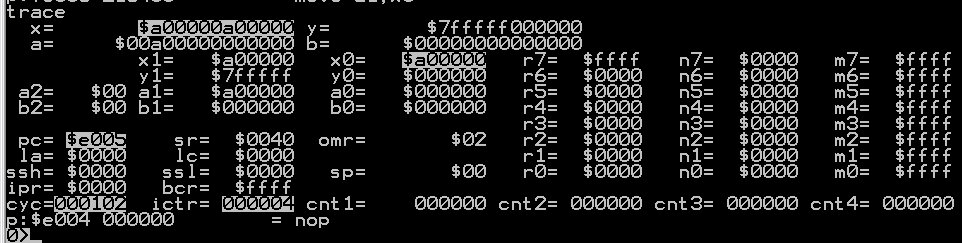
\includegraphics[width=\textwidth]{figs/ej3/3_4.png}
    \caption{Estado final de los registros (simulación).}
    \label{fig:ej3_simregs}
\end{figure}

